%%%%%%%%%%%%%%%%%%%%%%% TODO  %%%%%%%%%%%%%%%%%%%%%%%%%%%%%%%
% - Todas as páginas deverão ser contadas. Porém, as folhas pré-textuais (primeira até o sumário) não são numeradas. A numeração (contada continuamente) deverá figurar a partrir da Introdução até a última folha do trabalho, em algarismos arábico (resolvido utilizando set counter)
% - Colocar número de página no canto superior direito da página
% - Remover a página em branco depois do sumário (resolvdo quando mudei a classe de book para report)
% 
%
% Comentários de Rider:
% - Na introducao, expandir trabalhos prévios. Vender ideia e sua importância. 10 páginas de introdução. 
%


\documentclass[12pt]{report}

%%%%%%%%%%%%%%%%%%%%%%%%%% Packages %%%%%%%%%%%%%%%%%%%%%%%%

\usepackage[raggedright]{titlesec}
\usepackage[utf8]{inputenc}
\usepackage{graphicx}
\usepackage{wrapfig}
\graphicspath{{imgs/}{imgs/apx/}{imgs/ch1/}{imgs/ch2/}{imgs/ch3/}{imgs/ch4/}}
\usepackage[tc]{titlepic}
\usepackage{algorithm2e}
\usepackage[T1]{fontenc}
\usepackage{pdfpages}
\usepackage{setspace}
\usepackage[backend=biber, sorting=none]{biblatex}
\addbibresource{references.bib}
\linespread{1.3}

\usepackage[a4paper, left=30mm, right=20mm, top=30mm, bottom=20mm]{geometry}

\usepackage{times}

\usepackage{amsmath}


%%%%%%%%%%%%%%%%%%%%%%%% Personal Data %%%%%%%%%%%%%%%%%%%%%
\newcommand{\autor}{FERNANDO MARCOS WITTMANN}

\newcommand{\titulo}{OPTIMIZATION APPLIED TO NON-INTRUSIVE MONITORING OF RESIDENTIAL ELECTRICAL LOADS}

\newcommand{\titulobr}{OTIMIZAÇÃO APLICADA AO MONITORAMENTO NÃO INTRUSIVO DE CARGAS ELÉTRICAS RESIDENCIAIS}

\newcommand{\orientador}{Marcos Julio Rider Flores}

\newcommand{\ano}{2017}

\renewcommand{\contentsname}{Summary}

%%%%%%%%%%%%%%%%%%%%%%%% Thesis Text %%%%%%%%%%%%%%%%%%%%%%%%
\begin{document}

    %\pagenumbering{roman} 
    \pagenumbering{gobble}
    
    % Primeira folha  dando visibilidade à: Universidade, Unidade de defesa, Autor, Título na língua em que o trabalho foi redigido, título em português, local e data.




\thispagestyle{plain}


\includegraphics[width=7cm, height=3cm,keepaspectratio=true]{imgs/logo}
\begin{center}
  {
  
  \large\textbf{\textsc{UNIVERSITY OF CAMPINAS}}\\
  %\vspace{.5cm}
  \large\textbf{\textsc{SCHOOL OF ELECTRICAL AND COMPUTER ENGINEERING}}
%  \large\textbf{\textsc{DEPARTMENT OF SYSTEMS AND ENERGY}}
  
  %Faculdade de Engenharia Elétrica e da Computação
  }
\end{center}
\vfill
\begin{center}
  {\large\textbf{\textsc{\autor}}}
\end{center}
\vfill
\begin{center}
  {\Large\textbf{\textsc{\titulobr}}}
\end{center}

\vspace{0.5cm}

\begin{center}
  {\Large\textbf{\textsc{\titulo}}}
\end{center}


\vfill


\vspace{4cm}

\vfill
\begin{center}
  % O tamanho da fonte deve ser 12pt em negrito.
  % Deve-se utilizar caixa alta.
  \textbf{CAMPINAS \\ \ano}
\end{center}
    
    % Página de rosto dando visibilidade ao nome do autor; ao título do trabalho; ao nível (mestrado); a área de concentração; ao nome do orientador; ao local (cidade) e ao ano de depósito. Incluir informação assinada pelo Orientador de que o exemplar corresponde à redação final da tese/dissertação. 

\newpage

\thispagestyle{plain}


\includegraphics[width=7cm, height=3cm,keepaspectratio=true]{imgs/logo}
\begin{center}
  {
  \large\textbf{\textsc{FERNANDO MARCOS WITTMANN}}
  %\vspace{.5cm}
  
  }
\end{center}



%\vfill

\vspace{.5cm}

\begin{center}
  {\large\textbf{\textsc{\titulobr}}}
\end{center}


\begin{center}
  {\large\textbf{\textsc{\titulo}}}
\end{center}

\vfill

{\setstretch{1.0}
\vspace{1cm}
\begin{flushright}
  \begin{minipage}[c]{.5\textwidth}
    Dissertação apresentada à Faculdade de Engenharia Elétrica e da Computação (FEEC), da Universidade Estadual de Campinas como parte dos requisitos para a obtenção do título de Mestre em Engenharia Elétrica, na área de Engenharia Elétrica.
  \end{minipage}
\end{flushright}
%\vspace{1cm}

\begin{flushright}
  \begin{minipage}[c]{.5\textwidth}
Dissertation presented to the School of Electrical and Computer Engineering (FEEC) of the University of Campinas in partial fulfillment of the requirements for the degree of Master, in the area of Electrical Engineering. 
  \end{minipage}
\end{flushright}
\vspace{1cm}


%%%%% Linha
%\iffalse
\noindent
\textbf{Orientador: \orientador}
\vspace{.5cm}

\noindent
\begin{minipage}[c]{.5\textwidth}
  {\footnotesize\textsc{Este exemplar corresponde à versão final da dissertação
  defendida pelo aluno \autor, e orientada pelo Prof. Dr. \orientador.
  }}
\end{minipage}
\vspace{1cm}

\noindent
{
\vspace{1cm}
\noindent
\rule[1pt]{7cm}{.5pt}  % Linha para assinatura do orientador
}
\vspace{.5cm}
}

%\noindent
%\textbf{Orientador\ifx\femaleOrientador\undefined
%\else
%a\fi: \orientador
%}
%\vspace{.25cm}

%\ifx\coorientador\undefined
%\else
%\noindent
%\textbf{Coorientador\ifx\femaleCoorientador\undefined
%\else
%a\fi: \coorientador
%}
%\vspace{.5cm}
%\fi


%\noindent


%%%%%


\begin{center}
  {\small\textbf{\textsc{ Campinas \\ \ano}}}
\end{center}


    
    
    % Deve estar no verso da página de rosto. Quando se tratar de dissertações financiadas por agências de fomentos, os beneficiados deverão fazer referência ao apoio financeiro recebido e inserir, acima da ficha catalografica, além do nome da ag~encia, o número do processo pelo qual recebeu o Auxílio. 
    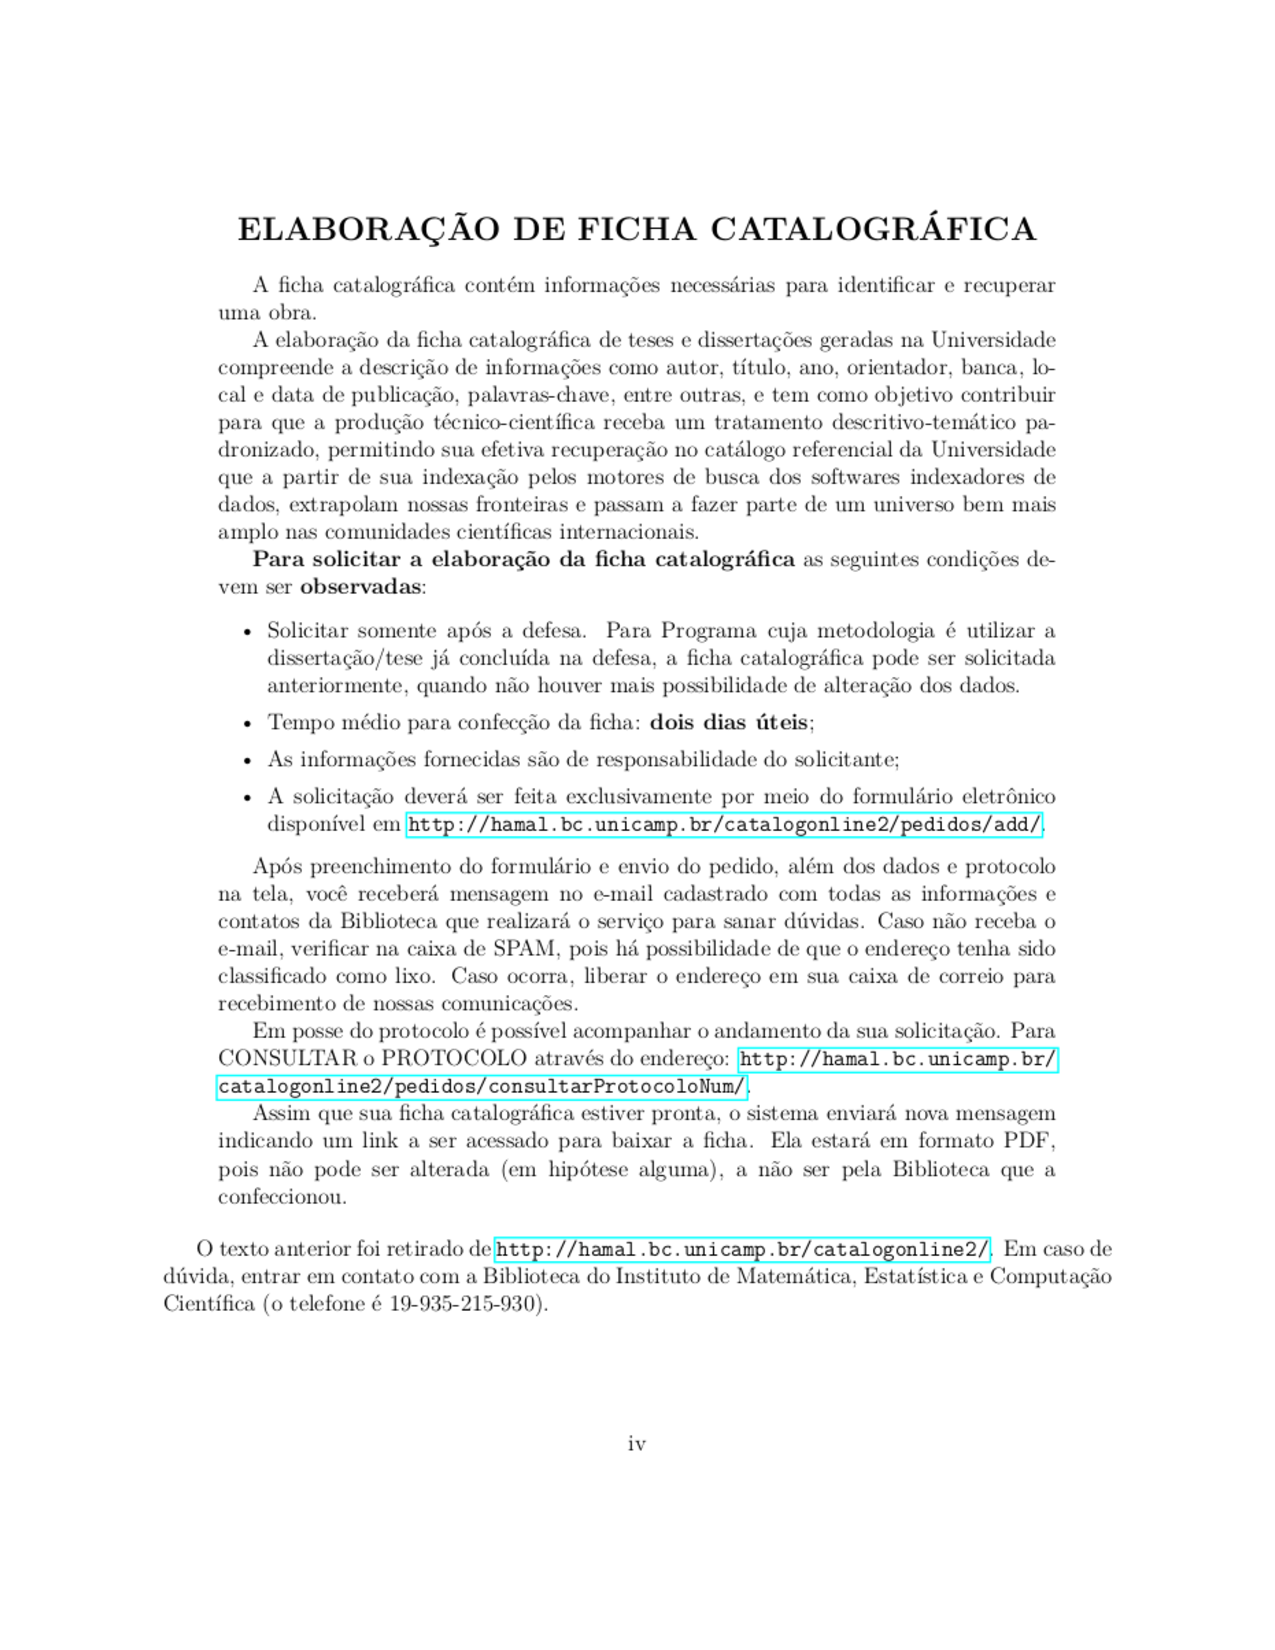
\includepdf{other/ficha-catalografica}
    
    % Folha de aprovação deve dar visibilidade à comissão examinadora com as respectivas assinaturas;
    %
\includepdf{other/folha-de-aprovacao}
    \newpage

\begin{center}
  \large{\textbf{COMISSÃO JULGADORA - DISSERTAÇÃO DE MESTRADO}}
\end{center}


{\setlength{\parindent}{0cm}

\vspace{2cm}


\textbf{Candidato:} Fernando Marcos Wittmann RA: 180577 \\
\textbf{Data da Defesa:} xx de setembro de 2017

\vspace{2cm}

\textbf{Título da Tese:} "Algoritmo de Monitoramento Não Intrusivo Utilizando Programação Linear Inteira Mista”.

\vspace{3cm}

Prof. Dr. Marcos Julio Rider Flores (Presidente, FEEC/UNICAMP)\\
Prof. Dr. Roberto Cayetano Lotero (CECE/UNIOESTE)\\
Prof. Dr. Nome do Outro Membro (FEEC/UNICAMP)\\

\vspace{3cm}

 A ata de defesa, com as respectivas assinaturas dos membros da Comissão Julgadora, encontra-se no processo de vida acadêmica do aluno.
 
}
    
    \newpage

\ \\
\ \\
\ \\
\ \\
\ \\
\ \\
\ \\
\ \\
\noindent
\begin{center}
    \textit{À meus pais, Ivo Amandio Wittmann e Maria Salete Wittmann.}
\end{center}
    
    \chapter*{Agradecimentos}%\markboth{Agradecimentos}{}}  % \markboth{}{} é utilizado para corrigir o cabeçalho.
%\phantomsection
%\addcontentsline{toc}{chapter}{Agradecimentos}
% FIXME Escrever os agradecimentos.


À meu orientador Marcos Rider pela oportunidade, orientação, confiança, paciência, apoio, contribuições, dedicação e disponibilidade. Sua abordagem como orientador tornou minha experiência de mestrado bastante motivante e agradável. \\
Aos colegas do LE19 e LE23, em especial ao Camilo Lopez pelas valiosas contribuições.\\
À meus amigos da república pelo companheirismo, em especial ao Nelson e ao Antônio, que me acompanharam desde os meus primeiros dias em Campinas. \\
À minha família. Meus pais Ivo e Salete e também meus irmãos Anderson e Andrea por sempre me apoiarem e pelo exemplo.\\
À FAEPEX pelo apoio financeiro.

%\iffalse


%\fi
    
    %\newpage

\vspace*{\fill}
{\raggedleft\vfill\itshape{
Quote\\
\ \\
}\par
Author\\
}
    
        
\newpage

\begin{center}
  \large{\textbf{RESUMO}}
\end{center}

% FIXME Remover deste ponto até a linha 14.
Este trabalho apresenta um método de monitoramento não intrusivo (Non-Intrusive Load Monitoring - NILM) baseado em programação linear inteira mista. NILM são métodos para decompor leituras de medidores de energia em informações a respeito dos aparelhos eletrodomésticos em operação. Tais informações, como consumo e estado de operação, são valiosas para promover a eficiência energética e manutenção preventiva. A técnica NILM proposta neste trabalho expande o modelo clássico fundamentado em otimização combinatória (Combinatorial Optimization - CO). A nova formulação lida com o problema de ambiguidade de cargas similares, presente no modelo clássico. Restrições lineares são utilizadas para representar eficientemente as assinaturas de carga. Além disso, uma estratégia baseada em janelas temporais é proposta para melhorar o desempenho computacional. A desagregação de cargas pode ser feita utilizando apenas medidas de potência ativa em uma baixa taxa de amostragem, disponível na maioria dos medidores de energia. A técnica é também adequada para uma abordagem sem supervisão. O desempenho do algoritmo é validado utilizando três casos de teste a partir da base de dados pública AMPds. Para a abordagem sem supervisão é utilizada uma base de dados residencial privada. A taxa de amostragem do caso de teste é de uma amostra por minuto. Os resultados demonstram a habilidade do método proposto para identificar e desagregar com precisão as assinaturas de energia individuais de forma computacionalmente eficiente. 

\vspace{.2cm}
\textbf{Palavras-chave}:
% FIXME Remover a linha abaixo.
desagregação de carga, assinatura de carga, programação linear inteira mista, monitoramento não intrusivo, otimização.
% TODO Inserir as palavras-chave aqui.

\vspace{3cm}
\newpage

\begin{center}
  \large{\textbf{ABSTRACT}}
\end{center}

This work presents a non-intrusive load monitoring (NILM) method based on mixed-integer linear programming (MILP). NILM are methods for decomposing measurements from energy meters into information regarding appliances in operation. Such information, such as the the power consumption and operating state, are valuable for promoting energy savings and predictive maintenance. The proposed technique expands the classical NILM combinatorial optimization (CO) model. The new formulation handles the problem of ambiguity of similar loads, present in the classic model. Linear constraints are used to efficiently represent load signatures. Additionally, a window-based strategy is proposed to enhance the computational performance of the proposed NILM algorithm. The disaggregation can be made using only active power measurements at low sampling rate, which is available at most energy meters. In addition, to improve the method's accuracy, other features can be added to the model, if available, such as reactive power or harmonic measurements. The technique is suitable to an unsupervised NILM approach. The performance of the algorithm is evaluated using three test cases from the public dataset AMPds. The unsupervised approach uses a private residential dataset. The sampling rate from the test case is 1 sample per minute. Results demonstrate the ability of the proposed method to accurately identify and disaggregate individual energy signatures in a computationally efficient way.


\vspace{.2cm}
\textbf{Keywords}:
% FIXME Remover a linha abaixo.
load disaggregation, load signature, mixed-integer linear programming, non-intrusive load monitoring, optimization.
    
    \newpage

\begin{center}
  \large{\textbf{LIST OF SIMBOLS}}
\end{center}


\noindent \emph{\textbf{Sets}}:


\vspace{4pt}

\begin{description}
    \item [{$D$}]           Set of appliances
    \item [{$S$}]           Set of indexes associated to power states
    \item [{$T$}]           Set of discrete time periods
    \item [{$\tilde{T}$}]   Subset of discrete time periods within a window, where $\tilde{T} \subseteq T$

\end{description}

\vspace{4pt}

\noindent \emph{\textbf{Indexes}}:

\vspace{4pt}

\begin{description}
    \item [{$i$}]   Index of each power state, where $i \in S$
    \item [{$j$}]   Index of each appliance, where $j \in D$
    \item [{$t$}]   Index of each time period, where $t \in T$

\end{description}

\vspace{4pt}

\noindent \emph{\textbf{Parameters}}:

\vspace{4pt}

\begin{description}

    \item [{$D_i$}]     Appliance associated with the state $i$
    \item [{$G_i$}]     Number of time periods in which the state $i$ must be activated
    \item [{$m$}]       Number of time periods in a window
    \item [{$MD_i$}]    Minimum number of time periods in which the state $i$ must be ON
    \item [{$n$}]       Total number of power states in $S$
    \item [{$NP_i$}]    Number of time periods in which $i$ has been activated in the previous window
    \item [{$P_i$}]     Active power state assigned to the index $i$
    \item [{$P(t)$}]    Active power true measurement at time $t$
    \item [{$\rm{prev}_\textit{i}$}]Previous state of $i$ (0 if none)
    \item [{$Q_i$}]     Reactive power state assigned to the index $i$
    \item [{$Q(t)$}]    Reactive power true measurement at time $t$
    \item [{$T_0$}]     Initial time period of each new window
    \item [{$T_f$}]     Last time period of each new window in $\tilde{T}$
    \item [{$T_{\text{end}}$}] Last time period of $T$ 
%    \item [{$TH$}]      Threshold of minimum power to be identified. 
    \item [{$X_i$}]     Final status of the state $i$ within the current window. $X_i=1$ if the state $i$ is ON at the end of the window; otherwise, $X_i=0$.

    \item [{$y_j(t)$}]     True power measurement of a given appliance $j$ at time $t$.
    \item [{$\hat{y}_j(t)$}]     Predicted power measurement of a given appliance $j$ at time $t$.

\end{description}

\vspace{4pt}

\noindent \emph{\textbf{Variables}}:

\vspace{4pt}

\begin{description}
    \item [{$dw_i(t)$}]         Binary variable that indicates if state $i \in S$ was turned off at time $t$
    \item [{$up_i(t)$}]         Binary variable that indicates if state $i \in S$ was turned on at time $t$ 
    \item [{$x_{i}(t)$}]        Binary variable that represents the status of state $i$ at time $t$
    \item [{$\delta_P(t)$}]     Difference between the measured value $P(t)$ and the combination of loads at time $t$
    \item [{$\delta_Q(t)$}]     Difference between the measured value $Q(t)$ and the combination of loads at time $t$
    
\end{description}

    
    \tableofcontents
    
    \listoffigures
 
    \listoftables

    \pagestyle{headings}

\chapter{Introduction}

\pagenumbering{arabic} 
\setcounter{page}{8}

\section{Motivation}

How much am I paying due to the energy consumption of my fridge? While simple, a typical homeowner do not have access to this kind of information yet. Providing energy usage feedback to homeowners is a helpful way for promoting the energy efficiency \cite{eci}. Detailed information on energy consumption is still invisible to the general population which implies in a source of waste. Without feedback, it is impossible for people to learn effectively about their energy usage patterns, necessary for energy savings. Unlike phone bills in which calls are individually identified, the energy bill shows only the total price which is a limited information. 

As shown in the spectrum of the Fig.~\ref{feedback}, the energy feedback can be either indirect or direct \cite{epri}: 

\begin{itemize}
\item The indirect feedback is provided after the consumption occurs. It may range from a standard electricity bill to daily reports. This is the most common scenario for customers of power utilities nowadays. 
\item The direct feedback is provided in real time with either aggregated or disaggregated energy information. As a difference, aggregated information provides the whole-building consumption information while disaggregated information provides appliance level consumption information.
\end{itemize}


Ideally, users should be able to access disaggregated feedback since more information to the user is provided and thus more control in their decisions. Disaggregated feedback is a valuable resource for homeowners, commercial buildings, and power utilities. For homeowners and commercial buildings, disaggregation helps them making decisions about their consumption habits and appliances to save energy \cite{CarrieArmel2013213}. In addition, it can be helpful to detect malfunctions, inefficient equipment or for scheduling predictive maintenance \cite{eunilm2016}. In regards to power utilities, disaggregation helps them to understand their customers and provide them with better-customized services \cite{eunilm2016-2}. However, disaggregated feedback is a very difficult task to be accomplished since it implies into finding a way to monitor all the appliances of a building. In fact, the disaggregation of loads can be accomplished either with intrusion or not intrusively:

\begin{itemize}
\item In an intrusive approach, it is connected one measurement device to each power outlet. This process might lead to high installation costs since it is necessary an infrastructure with one measurement device for each outlet and also a network infrastructure to connect all of them. This solution might also lead to privacy concerns, for example, if the power utility wants to provide an intrusive approach to theirs customers, their employees should go inside their customer's houses. 
\item On the non-intrusive approach, the energy consumption of the major appliances is estimated using only a single meter installed in the consumer’s energy input panel. The measurements acquired by the energy meter are processed in order to provide details about the operating devices.
\end{itemize}

The advantage of non-intrusive identification is the reduced costs of hardware, maintenance, and privacy. However, non-intrusive identification is still a software challenge due to the complexity of extracting a set of individual load measurements from the whole house power measurement. This challenge is closely related to the cocktail party problem where there are multiple sound sources recorded by a microphone and we want to extract just one of these sources \cite{ica}. In this context, non-intrusive load monitoring (NILM), also known as load disaggregation, is a research field which seeks to break down a whole-house power signal into individual devices.

\begin{figure}[tb]
    \centering
    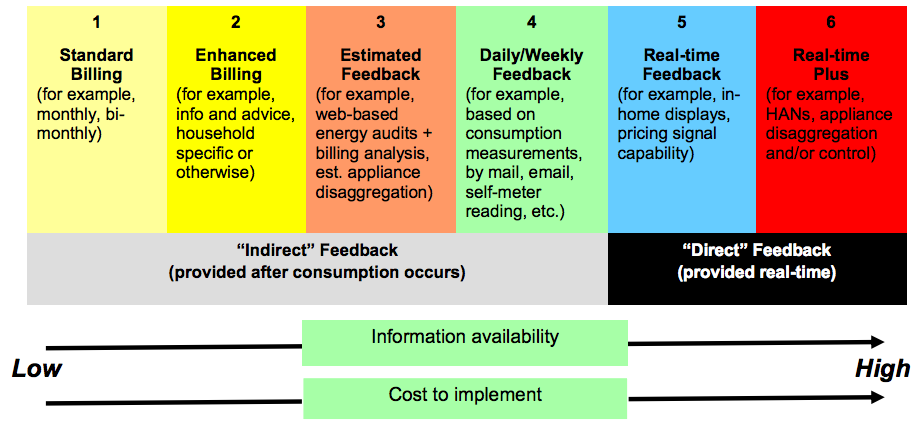
\includegraphics[width=1\columnwidth ]{feedback.png}
    \caption{Spectrum with the different types of energy feedback \cite{epri}}
    \label{feedback}
\end{figure}

\iffalse
How much energy did my fridge spend in the last month? While simple, a typical homeowner still do not have access to this kind of information. The number of energy meters in the world is expected to increase up to 780 Million by 2020 \cite{first}. However, unlike phone bills in which calls are individually identified and marked, the energy bill shows only the total price. No information about the consumption of each appliance is provided. Disaggregation of loads from power measurements is a valuable resource for homeowners, commercial buildings, and power utilities. For homeowners and commercial buildings, disaggregation helps them making decisions about their consumption habits and appliances to save energy \cite{CarrieArmel2013213}. In addition, it can be helpful to detect malfunctions, inefficient equipment or for scheduling predictive maintenance \cite{eunilm2016}. In regards to power utilities, disaggregation helps them to understand their customers and provide them with better-customized services \cite{eunilm2016-2}. The disaggregation of loads can be accomplished either with intrusion or not intrusively. In an intrusive approach, it is necessary to connect one measurement device to each power outlet, which leads to high installation costs and privacy concerns. On the non-intrusive approach, the energy consumption of the major appliances is estimated using only a single meter installed in the consumer's energy input panel. The advantage of non-intrusive identification is the reduced costs of hardware, maintenance, and privacy. In this context, the objective of non-intrusive load monitoring (NILM), also known as load disaggregation, is to break down a whole-home power signal into individual appliances.
\fi

\section{Description of the Problem}

The keyword NILM was introduced in 1985 by George W. Hart in a technical report \cite{hart85} and later published in 1992 by the same author \cite{hart}. The paper proposes a full methodology, from types of loads, load signatures, algorithm and physical implementation. The algorithm is based on pattern recognition, which is described in the next chapter. 

Before introducing the pattern recognition method, Hart describes the NILM problem as a combinatorial optimization (CO) problem. However, the author discourages its usage as described below. In the CO formulation, the disaggregation is obtained by combining the multiple possible states that minimizes the full measurement for each time instant. For each time instant, we seek to minimize the error between combination of power states and the aggregated measurement. Here, it is assumed that all the possible operating states are previously known. More details about this formulation is also presented in the next chapter. Hart points three main issues to discourage the usage of this formulation: 
\begin{itemize}
\item The problem has a high computational cost and it increases with the addition of more states of devices or measurements.
\item \textbf{Fundamental Problem}: The complete set of operating states are never known. If the model is used in the presence of unknown appliances, it would attempt to describe their behavior as a combination of other known appliances. 
\item \textbf{Multiple Switching (MS)}: A small change in the measurement might be translated into a big change of the combination of loads. 
\end{itemize}
As shown in the next section, despite various NILM approaches proposed in the literature, very few have attempted in dealing with the CO formulation. While those difficulties are still challenging, there is still room and potential for expanding the formulation in ways to handle the previous problems. This work is especially concerned in solving the MS problem and decreasing their running time of the algorithm. 
%The fundamental problem may also be handled with preprocessing techniques, as shown in the Section 4.  


\section{Previous work}

Figure \ref{1npub} shows the number of publications in the NILM field per year over the last 25 years. Those NILM publications are inferred using publications citing the first NILM work published by Hart in 1992\footnote{Based on \cite{1npub}. Data acquired from Google Scholar. Code available in \url{https://github.com/WittmannF/nilm-publications}}. An exponential growth of NILM publications can be observed since 2010.

\begin{figure}[bt]
    \centering
    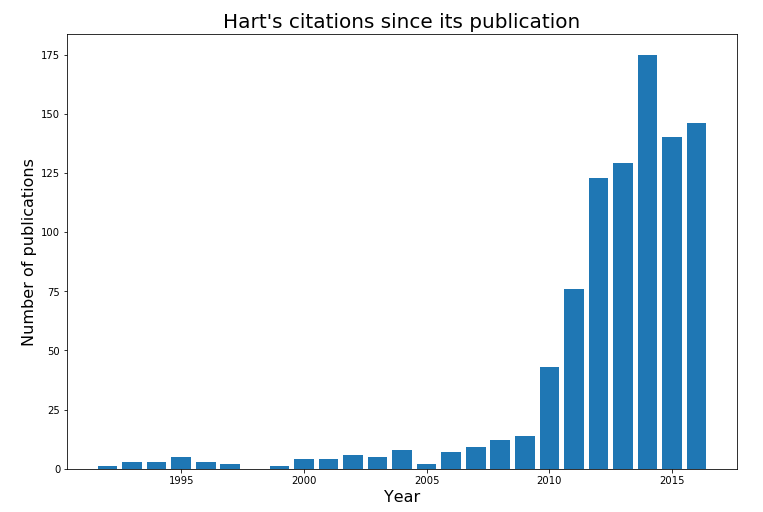
\includegraphics[width=0.8\textwidth]{npub}
    \caption{Number of publications with reference to Hart's original work since its publication}
    \label{1npub}
\end{figure}


%The second problem led the author to propose the switch continuity principle (SCP), which states: \textit{``In a small time interval, we expect only a small number of appliances to change state in a typical load''}. However, as shown in recent works \cite{makonin2016}, SCP is not always reliable. Hence, a better strategy to deal with MS is necessary.
A further analysis in the publication's titles since 2010 did not reveal any trending strategy. Figure \ref{wordle} shows the most frequent words in those titles. Some obvious keywords such as 'nonintrusive', 'load', 'monitoring', 'energy' and 'disaggregation' were removed. As main insights, the NILM research field seems to be mainly focused in residential applications and buildings. Therefore, few attention has been paid to industrial applications. In addition, it seems that privacy is increasingly a concern in the field.

\begin{figure}[bt]
    \centering
    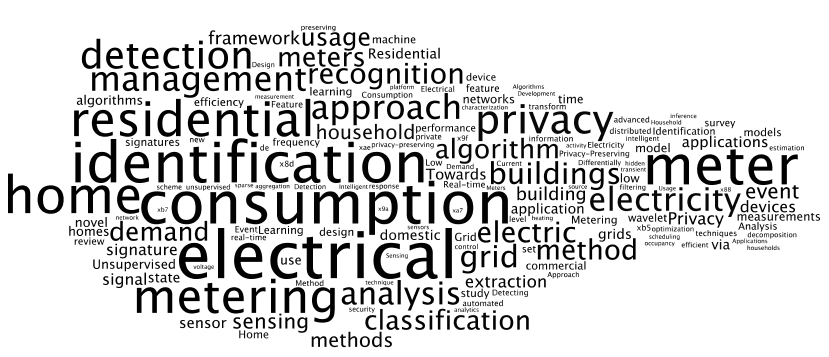
\includegraphics[width=0.8\textwidth]{wordle}
    \caption{Trending words in the titles of NILM publications since 2010}
    \label{wordle}
\end{figure}

There are many ways of categorizing the NILM approaches. For example they can be categorized into either supervised or unsupervised approaches \cite{makonin2016}:

\begin{itemize}
    \item Supervised NILM uses measurements of each single appliance to build their models and then disaggregate. It is assumed that we previously have access to the measurements of each individual appliance that is part of the full house measurement. 
    \item Unsupervised NILM does not require single measurements of each appliance for training. This approach allows general appliance models as input which are then tuned to each specific house. The challenge here is to find the right parameter's values to be tuned. 
\end{itemize}

Zeifman and Roth in \cite{zeifman} divide the types of algorithms in two categories: pattern recognition (one-to-one matching) and optimization (multiple matching). Zeifman's categorization could also be expanded into either event-based algorithms or eventless algorithms:

\begin{itemize}

    \item The event-based  matching  is  based  on  the  detection  and  classification  of  events. Since the pattern recognition strategies are based on one-to-one matching, the efforts of these strategies are mainly focused on feature extraction. As example of features to be extracted we have the active and reactive power, harmonics, wavelet's signatures and fundamental frequency. These events are then classified by well-established classifiers, such as k-nearest neighbor \cite{Figueiredo2011, berges2009, Froehlich2010}, fuzzy sets \cite{lin2011, ducange2014}, decision trees \cite{Nguyen2015, gillis2016}, support vector machines \cite{duarte2012, zoha2012}, neural networks \cite{zhou2016, bian2016} and deep learning \cite{mauch2016, jack2015}. As noted by \cite{zeifman}, the advantages of pattern recognition methods are that they provide better results in the presence of unknown loads. However, those methods are sensible to the detection of false edges coming from noise or non-linear loads.
    
    \item Eventless methods are based on the simultaneous matching of multiple loads, and they find the set of energized appliances that best fit the measured load. Most efforts from researchers on this side are given methods based on probabilistic models such as hidden Markov models (HMM) \cite{afhmm, reed, hmm_unsup, stephen_hmm}. Other approaches includes sparse coding \cite{sparse_kolter, nmf}, genetic algorithms \cite{meta} and integer programming \cite{suzuki, bhotto2016}. These methods provide better disaggregation performance \cite{zeifman} and are less sensible to edge detection. However, they are more susceptible to the fundamental problem presented in the previous section. 

\end{itemize}


Regarding the programming approaches,\footnote{Both the terminologies optimization and (mathematical) programming are equivalent and are going to be used interchangeably in this work} very few of them were focused on expanding the classical CO model. Some of these works are going to be discussed in the next subsection.  

\subsection{Related Work based on Optimization}

% Egarter and Elmenreich in \cite{meta} verify the MS problem by evaluating six meta-heuristics to solve the CO problem formulated as a knapsack problem. 
\cite{meta} shows the CO pointed in Hart's paper and discusses their equivalency with the knapsack problem. In short, it states that the classic equation is equivalent to the knapsack problem presented in \ref{knap} with a profit $d$ of 1 for all loads, and considering the capacity $C$ corresponds to the total load $P(t)$. However their paper is focused on verifying Hart’s statement regarding the MS. Five metaheuristics optimization approaches are evalutated. Their work does not expand the the appliance model, such as new constraints to enhance the identification accuracy. They conclude that it is hard to disaggregate loads with similar power drawns and proposes as future work a multi-objective optimization approach.

\begin{equation} \label{knap}
   max \quad \sum_{i=1}^{n} d_i \ x_i
\end{equation}

$$ s. \ t. \quad \sum_{i=1}^{n} w_i \ x_i \leq C $$

Kolter and Jaakkola in \cite{afhmm} formulate the NILM problem as a convex quadratic programming problem. The authors consider an extension to HMMs, called additive factorial hidden Markov models. Furthermore, authors in \cite{afhmm} describe an unsupervised learning procedure. However, the method needs a regularization parameter that changes for each problem. In addition, the optimization function is made over the full set of time periods, which make the method computationally expensive.

\cite{suzuki} formulates the NILM problem as an integer quadratic programming problem. The technique represents the problem, as a combination of waveforms from multiple loads. 
At any given one period of current, the overall load current is represented as a superposition of each current of the operating appliance. The overall current waveform is considered to be influenced by the waveform of each individual appliance as shown in the Figure \ref{1suzuki}. However, it requires very high frequency data. The model is based on the reading of one cycle (60Hz or 50Hz), so a large number of points from each cycle is necessary. In addition, as mentioned by Zeifman in \cite{zeifman}, the approach is somewhat naive since features are usually more robust than just unprocessed waveforms.


\begin{figure}
    \centering
    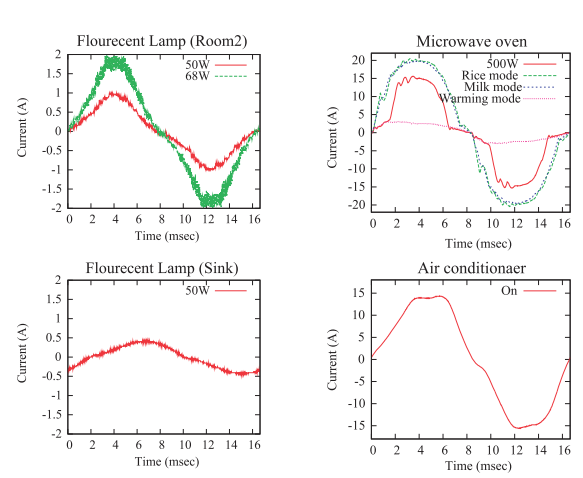
\includegraphics[width=0.8\textwidth]{1suzuki}
    \caption{Example of current waveforms for different loads, used by \cite{suzuki}}
    \label{1suzuki}
\end{figure}

Finally, authors in \cite{bhotto2016} propose a load disaggregation method based on integer linear programming. The work proposes enhancements to CO, such as state transition diagram and median filtering, to deal with the MS. Most enhancements in \cite{bhotto2016} are included as an intensive preprocessing rather than constraints. In addition, their model relies only on instantaneous load samples. Hence, their model is limited to the usage of constraints that does not depend on time measurements.

\section{Objectives}

Based on the efforts made by previous works, the goal of this work is to represent and solve the NILM problem as a mixed-integer linear programming (MILP) problem. We are especially concerned on expanding the classic CO problem in order to deal with complex load signatures. The CO formulation was not very much explored in previous works and we seek to propose new constraints for optimizing the identification of loads. In addition, this investigates strategies to improve the running time of the problem, which is also one of its main weakness. Another objective of this work is to compare the proposed formulation with classic works. Most previous works are based on either event based techniques or probabilistic models and this work allows researcher to expand the range of possibilities and approaches.

%The contributions of this work are brought from (). The work deals with the unit commitment problem in which try to allocate multiple combination of termal units for a given period. The constraints for modeling time and x demonstrates to be useful for NILM . 

\section{Contributions}

The main contributions of this paper are as follows:

\begin{itemize}
\item The NILM problem is represented as a MILP model, in which a new set of integer linear constraints is proposed to efficiently model the load signatures of the appliances.
\item In order to enhance the computational performance, the proposed NILM is solved using a window-based algorithm in which the overall problem is segmented into small, coupled sub-problems that can be efficiently solved via commercial MILP solvers.
\item The proposed model is also suitable for unsupervised NILM in the context described in \cite{makonin2016}. The model relies in parameters that can be acquired from aggregated data, such as, minimum operation time and sequence of states.
%\item A new set of constraints to model the load signature
%\item A window based algorithm in order to make the algorithm to run more efficiently
%\item The problem that led Hart to propose the \textit{switch continuity principle} is avoided in the tests cases
\end{itemize}

\section{Organization of the Work}

The next sections of this dissertation goes in this way:
\begin{itemize}
\item The Chapter 2 describes the background work that is used as basis for the remaining chapters. The reader may skip subsections that are already familiar with. 
\item The Chapter 3 describes the main contributions of this work. A math model for modeling the load signature. 
%\item The Chapter 4 describes the process of extracting the features that are used for feeding the input table of the model. The chapter is divided into two subsections: A supervised approach which uses clustering for extracting the main information and an unsupervised approach which is based on edge detection and histogram analysis.
\item The Chapter 4 describes the test cases with results for both the unsupervised setting and the supervised one. 
\item Finally, the Chapter 5 presents the main conclusions and future work. 
\end{itemize}
    
    \chapter{Fundamentals}
This chapter presents the fundamental concepts 


\section{Mathematical Optimization}

\iffalse
However, before introducing the pattern recognition method, Hart describes the NILM problem as a combinatorial optimization (CO) problem, formulated in the following way: let's assume that the measured value (current/power) in the input of the house is $P(t)$ at time $t$. The goal of the algorithm would be to decode $P(t)$ in many components $P_i(t) \ \forall \ i \in 1..n$, where $n$ is the number of power components and each one would be be associated to one specific state $i$. Hence, we have that

$$P(t) = P_1(t) + ... + P_n(t)$$
 
The CO formulation can be written by using the equation \ref{co} for each time reading $t$ 

\begin{equation} \label{co}
    \min_{x} \quad \left|P(t) - \sum_{i=1}^{n} x_i\ P_i \right|
\end{equation}

where $x_i(t)$ is a boolean that describes the state of the power component $i$ at time $t$. As noted in the reference, this problem although mathematically attractive, is a NP-complete “weighted set” problem, hence it has a high computational cost. In addition, it's complexity increases with the addition of more states of devices or measurements.
\fi


Mathematical optimization (also known as mathematical programming) is the process of minimization or maximization of an objective function of many variables, subject to constraints on the variables \cite{ampl}. The equation \eqref{opt_example} shows an example of optimization problem.

\begin{equation} \label{opt_example}
    \max_{x_i} \quad \sum_{i\ = 1}^{n} v_i\ x_i
\end{equation}

subject to 

\begin{equation}
    \sum_{i\ = 1}^{n} w_i\ x_i \ \leq \ W \quad \forall \ x \in \{0,1\}
\end{equation}

Equation \eqref{opt_example} is a classic \textit{integer programming} problem also known as the knapsack problem. Given a set of $i = 1..n$ different items, where each item has a specific value $v_i$, the main goal is to maximize the overall profit given that each item has a weight $w_i$ and it is not possible to overcome the maximum limit $W$. The variable of this problem $x_i$ is an integer binary variable, hence, the name of this type of problem. Some of the major subfields for mathematical optimization are \cite{cplex, ampl}:
\begin{itemize}
    \item \textbf{Linear Programming:} In this type of problem, the variables in the optimization function and in the constraints are linear. In the constrains, those variables are always assumed to be a linear combination of other variables. In the optimization funciton, the variables are always first order equations.  
    \item \textbf{Nonlinear Programming:} The objective function and/or the constraints contain nonlinear variables. A nonlinear variable could be a convex problem, for example, minimize the square of an error between. The product of two variables is also considered a non linear formulation. 
    \item \textbf{Integer Programming:} Linear problem in which all the variables are assumed to take an integer value. This value could be either a binary value or an natural number. 
    \item \textbf{Quadratic Programming:} Allow quadratic terms in the objective function. Most times, this is a convex problem.
    \item \textbf{Mixed-Integer Linear Programming:} Integer programming problem which contains a linear objective function (without quadratic terms).
\end{itemize}

\cite{cplex}. 

\subsection{Optimization Software}
ampl
gams
knitro
cplex

\subsection{Linearization of an Absolute Objective Function}
Boyle in cite{boyle} demonstrates how to linearize the \textit{Chebyshev approximation problem} defined as:

\begin{equation} \label{chebyshev}
    \min_{x} \max_{i=1,...,k} \quad \left| a_i^T\ x - b_i \right |
\end{equation}

\section{NILM as a Combinatorial Optimization Problem}

The energy disaggregation problem can be formulated assuming that the measured variable (current or power) in the input of the house is given by $P(t)$, for each time $t$. As shown in \eqref{Ps}, the objective of the NILM would be to decode $P(t)$ in power states $P_i(t)$, $\forall \ i \in \{1,...,n\}$. Where $n$ is the total number of power states for all appliances. 

\begin{equation} \label{Ps}
    P(t) = P_1(t) + ... + P_n(t)
\end{equation}
 
Each appliance is associated with one or more power states. For example, an ON/OFF appliance (e.g., a toaster) could be represented by a single state, while a washing machine could be represented by multiple states, since its power consumption changes over time. 
Eventually, the classical NILM problem can be rewritten as the optimization problem shown in the equation \eqref{classic}. Where $x_i(t) \in \left\{ 0 , 1 \right\}$ is a boolean variable that decides the status of the power state $i$, at time $t$ \cite{hart}.

\begin{equation} \label{classic}
    \min_{x} \quad \left| P(t) - \sum_{i=1}^{n} x_i(t)\ P_i \right |
\end{equation}

Equation \eqref{classic} aims at finding the combination of power states $P_i$ that best approximate the measure $P(t)$. When other types of measurements are also available (such as reactive power, harmonics or distortion factor), the classical problem in \eqref{classic} may include these measurements in a vector. Equation \eqref{classic2} also includes the reactive power measurement $Q(t)$ and reactive power states $Q_i$. 

\begin{equation} \label{classic2}
    \min_{x} \quad \left|\ \begin{bmatrix}
         P(t) \\
         Q(t) \\
        \end{bmatrix} - \sum_{i=1}^{n} x_i(t)\ \begin{bmatrix}
         P_i \\
         Q_i \\
        \end{bmatrix} \ \right|
\end{equation}

While the author x mentions that this approach is not viable due to the explosion of features, i.e., high computational time, the author considered a scenario in which the input table contains over x inputs. As described later, this work does not requires a big number of features and it runs in a fair computational time. In addition, there are constraints for atenuating the computational influence. 

\iffalse
Responder à estas críticas:


- Optimisation is computationally intractable
George Hart, one of the early pioneers of disaggregation research, points out that the optimisation
problem specified in equation 7.2 is an NP-complete “weighted set” problem and that
a precise solution is only achievable by enumerating every possible state (G. W. Hart 1992).
This is computationally impractical because n appliances, each of which can occupy any one
of s states, can be configured in s
n
combinations so the computational complexity blows up
exponentially as O(s
n
). Say we have thirty appliances, each of which can be in one of four
states, and we have a month of data sampled once every five seconds. That is approximately
1024 operations1
, which would take 5×1010 seconds (∼ 1 700 years) on NVIDIA’s top-of-the-line
GPU at the time of writing2
.
Whilst the optimisation problem specified in equation 7.2 is a succinct description of the problem,
it fails to capture many of the challenges present in practical systems. These problems
include (but are not limited to):
1. We are unlikely to know the power consumption of every appliance.
2. We are unlikely to know the total number of appliances.
3. Many appliances do not draw tidy, discrete levels of power; instead their power consumption
may spike, undershoot, oscillate or ramp over time.
4. A smart meter may sample less frequently than is required to faithfully capture rapid
changes. In other words, the meter may sample at sub-Nyquist rates. This results in
considerable distortion of the digital recording.
5. Many appliances (like washing machines and tumble driers) have multiple internal states.
Transitions between these states may be non-deterministic. Each run of the appliance
may produce a different waveform (see Figure 7.1).
6. Different appliances of the same class produce different waveforms (which is a problem if
we want to build a common database of appliances for multiple users).
7. Some appliances generate identical waveforms (e.g. a kettle and the water heater in a
washing machine generate very similar waveforms).
8. Appliance signatures overlap and occlude each other in the aggregate smart meter signal.
9. The mains voltage in the UK is nominally 230 volts but can range from 216 volts to
253 volts which is -6%, +10% of the nominal 230 volt supply voltage3
. Assuming a linear
load, we can expect the power consumption to vary by -12%, +20%. Home energy meters
do not measure voltage, but utility-installed smart meters do.
10. Ultimately users care more about how much energy each appliance uses rather than when
each appliance is on. Estimating energy consumption for a simple two-state appliance
like a toaster is trivial if we know how long the appliance has run for. But estimating
power consumption of complex appliances like washing machines is less trivial.
These challenges mean that conventional optimisation approaches such as combinatorial optimisation
are not feasible for anything other than toy scenarios.


\fi

\section{Pattern Recognition}
- describe
- figures 

\section{NILM as a Pattern Recognition Problem}
One of the most popular approaches for solving the NILM problem is pattern recognition. The technique is fundamentally based on finding pairs of edges in the signal with opposite directions. The figure x describes the first algorithm, proposed by Hart in x. 

\section{Other Approaches}
- HMM


Most of the successive works were focused on alternative edge detection strategies and increasing the number of features to be used besides the active and reactive power from the original work. Those alternative features includes harmonics, time of operation, hour of activation, etc. There are also features extracted from high frequency data such as the senoidal signal. However, it is worth noting that many of those features are not available in smart meters. Hence, NILM strategies should also be suitable to cases with limited data. 

\section{Summary}
    
    
\chapter{Math Load Model}

%[MOTIVACAO]
The previous chapter described the major background, necessary for the rest of this work. As shown in the introduction, very few progress was observed in the CO formulation. This chapter proposes new constraints and strategies for expanding the CO model. We are especially interested in constraints for modeling the signature of a load and improve its performance. First, a visual intuition will be introduced. Next, the classic NILM optimization problem is reformulated as a MILP problem. Then, three constraints are proposed for defining a load signature such as the transition of states and minimum time. Strategies and constraints for decreasing the computation time are also introduced. Finally, the full proposed model is presented. 

\section{Visual Intuition}
- The fig

\section{Mixed-Integer Linear Programming (MILP) Formulation}

The Equation \eqref{classic2} can be reformulated as a MILP problem, shown in \eqref{milp2}--\eqref{eq7}. This way, the new formulation becomes suitable for linear solvers.

\begin{equation} \label{milp2}
    \min_{x_i(t)} \quad \sum_{t\ \in\ T} \delta_P(t) + \delta_Q(t)
\end{equation}

subject to 

\begin{equation} \label{eq65}
    P(t) - \sum_{i\ = 1}^{n} x_i(t)\ P_i \ \leq \ \delta_P(t) 
\end{equation}

\begin{equation} 
  P(t) - \sum_{i = 1}^{n} x_i(t)\ P_i \ \geq \ -\delta_P(t)
\end{equation}

\begin{equation} 
   Q(t) - \sum_{i\ = 1}^{n} x_i(t)\ Q_i \ \leq \ \delta_Q(t)
\end{equation}

\begin{equation} \label{eq7}
  Q(t) - \sum_{i = 1}^{n} x_i(t)\ Q_i \ \geq \ -\delta_Q(t)
\end{equation}

Where $\delta_P(t)$ and $\delta_Q(t)$ in \eqref{milp2} are the difference between the aggregated power states and the actual measurement (i.e., the approximation error). Besides the linear formulation, another difference from \eqref{classic2} is that the time $T$ is included in the objective function. The advantage of doing this is the possibility of adding new time-dependent constraints in order to improve the model's accuracy. 

\subsection{Window-based formulation}
The time set $T$ increases the computational burden since the variable $x_i(t)$ depends on the number of time periods. To overcome this issue, it is possible to separate the set of time periods into smaller, homogeneous windows. Let $\tilde{T} \subset T$ be the set of time periods within a window, where $\tilde{T} = \left\{ T_{0} , T_{0} + 1, \cdots , T_{0} + m \right\}$, $m$ is the number of time steps of the window, and $T_{0}$ is the initial period for each window. The MILP problem can now be written using a sequenced  optimization process as shown in Algorithm \ref{algorithm1}, where $T_{\text{end}}$ is the final period of $T$.

\begin{algorithm}\label{algorithm1}
\SetAlgoLined
 \Repeat{$T_{0}$ > $T_{\text{end}}$}{

let  $\tilde{T} = \left\{T_{0}, \cdots, T_{0}+m \right\}$

solve
\begin{equation}
    \min_{x_i(t)} \quad \sum_{t\ \in\ \tilde{T}} \delta_P(t) + \delta_Q(t)
\end{equation}

s.t.:

\begin{equation} \label{first_eq}
    P(t) - \sum_{i = 1}^{n} x_i(t)\ P_i \ \leq \ \delta_P(t)
\end{equation}

\begin{equation}
  P(t) - \sum_{i = 1}^{n} x_i(t)\ P_i \ \geq \ -\delta_P(t)
\end{equation}

\begin{equation} \label{third_eq}
    Q(t) - \sum_{i = 1}^{n} x_i(t)\ Q_i \ \leq \ \delta_Q(t)
\end{equation}

\begin{equation} \label{fourth_eq}
  Q(t) - \sum_{i = 1}^{n} x_i(t)\ Q_i \ \geq \ -\delta_Q(t)
\end{equation}


let $T_0 = T_0 +m +1$
 }
 \caption{NILM using a window-based algorithm}
\end{algorithm}

Algorithm 1 is still equivalent to the classic optimization formulation and will be used as one of the approaches to be compared in the results. From now on, Algorithm 1 will be referred as the CO method. 

One more constraint that is helpful for cases in which the reading in the window is less than a given threshold (for example $TH = 30W$). The constraint \eqref{set_zero} allows to automatically set to zero the binary variables under those circumstances. 

\begin{equation} \label{set_zero}
   x_i(t) = 0 \quad \forall t \in \tilde{T}, i \in S | P(t) \leq TH
\end{equation}

\section{Load Signature Constraints}

In this section, a new set of constraints are presented to model the load signatures and to communicate the optimization process of one window with the others. First, let's consider a practical example. Fig.~\ref{example} shows the load signature of two hypothetical appliances: a washing machine and a stove.

\begin{figure}[tb]
    \centering
    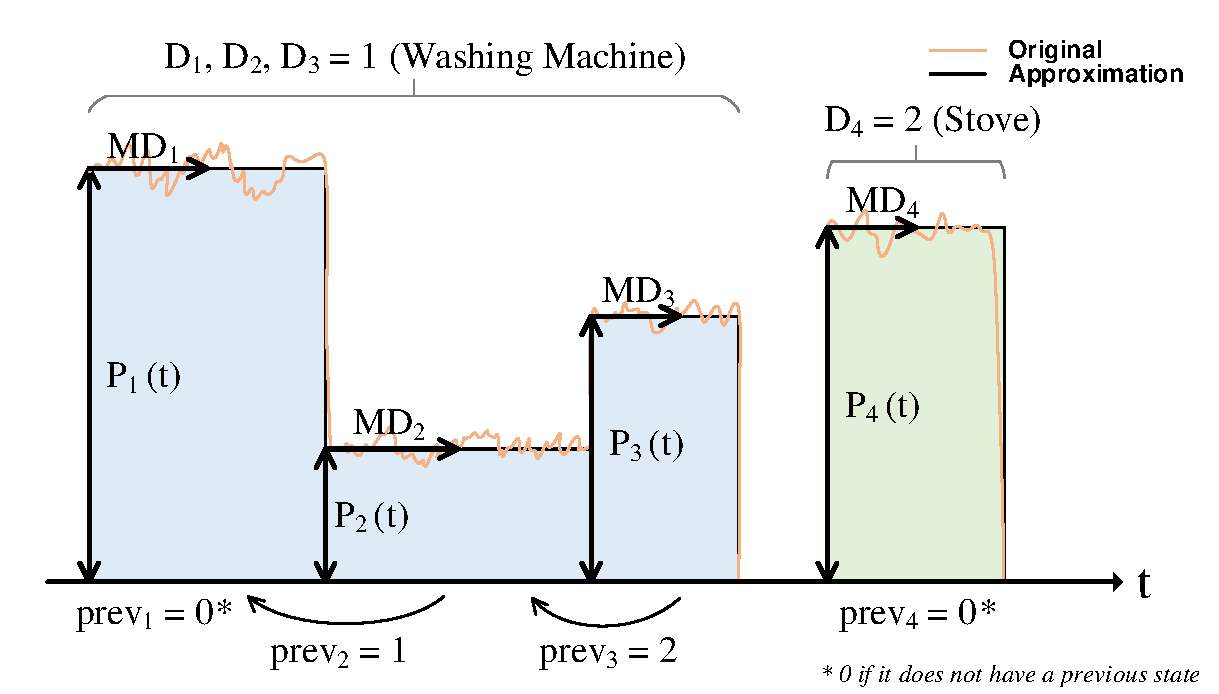
\includegraphics[width=1\columnwidth ]{example_2.pdf}
    \caption{Two hypothetical load signatures to be modeled}
    \label{example}
\end{figure}

The washing machine's load signature can be approximated using three power states ($P_1(t)$, $P_2(t)$ and $P_3(t)$) while the stove's has one single power state ($P_4(t)$). In order to model these loads, the following hypotheses are considered: 

\begin{itemize}

\item Multiple states $P_i(t)$ (also multiple reactive power states, if available) from the same appliance cannot be activated simultaneously;
\item Some loads work as finite-state machines, i.e., a given state is only activated if another state of the same appliance has finished;
\item A state $i$ can have a minimum time $MD_i$ in which it should remain ON.

\end{itemize}

The former hypotheses are used to formulate a set of constraints used to efficiently represent the load signatures within the proposed MILP model. A detailed analysis of each one of the former hypotheses is shown in the following subsections.

\subsection{Avoiding Multiple States From the Same Appliance}

Parameter $D_i$ identifies the appliance's index of each state $i$. For example, the states $i = 1, 2, 3$ in Fig.~\ref{example} are associated to the washing machine, that is, $D_1 = D_2 = D_3 = 1$, where the number 1 means ``washing machine''. Likewise, $D_4$ refers to the stove, identified by the number 2. In order to avoid simultaneously allocation of different power states from the same appliance, constraint \eqref{overl} can be included.

\begin{equation} \label{overl}
   \sum_{i \in S | D_{i} = j} x_i(t) \leq 1 \quad \forall t \in \tilde{T}, j \in D
\end{equation}

Constraint \eqref{overl} limits the sum of the states $x_i(t)$ from the same appliance to one. This way, $x_1(t)$, $x_2(t)$ or $x_3(t)$ cannot be simultaneously activated since $D_1$, $D_2$ and $D_3$ are associated to the same appliance.

\subsection{Linking the Transition Between Power States}

In Fig.~\ref{example}, power state $P_2(t)$ should be ON only if the power state $P_1(t)$ has finished. Likewise, we could also fix the power state $P_3(t)$ to be ON only if $P_2(t)$ has finished. The goal is to include a constraint that allows a specific power state to be activated only if a previous one (from the same appliance) has finished. To do so, two binary variables are used to determine the transition from a ON state to an OFF state, and vice versa. The two variables are called $up_i(t)$ (turned ON) and $dw_i(t)$ (turned OFF). Then, the linking constraints are given by \eqref{updw}--\eqref{updw2}.
%
%\vspace{-10pt}

\begin{equation} \label{updw}
    x_i(t) - x_i(t-1) = up_i(t) - dw_i(t) \quad \forall i \in S, t > T_0
\end{equation}


\begin{equation} \label{updw3}
    x_i(T_0) - X_i = up_i(t) - dw_i(t) \quad \forall i \in S, t = T_0
\end{equation}

\begin{equation} \label{updw2}
    up_i(t) + dw_i(t) \leq 1 \quad \forall i \in S, t \in \tilde{T}
\end{equation}

\noindent where $X_i$ saves the state $x_i(t)$ of the last time period of each window, necessary for the initialization of $x_i(t)$ in the next window. In constraint \eqref{updw}, $up_i(t)$ will be 1 only if the decision variable $x_i(t)$ makes a transition from 0 to 1, at time $t$. Likewise, $dw_i(t)$ will be 1 only if $x_i(t)$ makes a transition from 1 to 0, at time $t$. Next, \eqref{updw3} links the state transitions between windows. Finally, \eqref{updw2} prevents $up_i(t)$ and $dw_i(t)$ to be simultaneously 1.

%Now that we have these two variables, let's consider that we save the transition of states in a parameter called $\text{prev}_i$. In the Fig. \ref{example} we have for example in the washing machine that the value of $prev_2$ is 1 since we want to fix the second state to happen only after the first one. We can fix state transitions using the following constraint:

Using constraints \eqref{updw}--\eqref{updw2} and the parameter $\text{prev}_i$, we can now link the transition between two states using the additional equation in \eqref{state}.

\begin{equation} \label{state}
    up_i(t) = dw_{\text{prev}_i}(t) \quad \forall i \in S, t \in \tilde{T} \ | \ \text{prev}_i>0
\end{equation}

As an example, the state $i = 2$ of the washing machine in Fig.~\ref{example} can only change from OFF to ON (i.e., $up_2(t) = 1$) if the state $i = 1$ has change from ON to OFF (i.e., $dw_1 = 1$), at a given time $t$.

\subsection{Minimum Active Time}

One last hypothesis that is proposed in this paper is setting a minimum active time of a state. Parameter $MD_i$ in Fig.~\ref{example} establishes the minimum number of time samples in which the state $i$ should be kept activated. The set of constraints presented in \eqref{md1}--\eqref{md3} are proposed to carry out this process. 

\begin{equation}\label{md1}
    \sum_{k\ =\ T_0}^{G_i} \left[ 1 - x_i(k) \right] = 0 \quad \forall i \in S
\end{equation}

\begin{multline}\label{md2}
    \sum_{k\ =\ t}^{t+MD_i-1} x_i(k) \geq MD_i \left[ x_i(t) - x_i(t-1) \right] \\
    \forall i \in S, t \in G_i + T_0 \hdots T_f - {MD}_i + 1
\end{multline}

\begin{multline} \label{md3}
    \sum_{k\ =\ t}^{T_f} \left\{ x_i(k) - \left[ x_i(t) - x_i(t-1) \right] \right\} \geq 0 \\
    \forall i \in S, t \in T_f - MD_i + 2 \hdots T_f 
\end{multline}

Constraint \eqref{md1} activates a certain state that was already activated at the end of the previous window, but for less than $MD_i$ samples. Parameter $G_i$ is the number of periods in which the state $i$ must remain ON at the beginning of the window. It is calculated as $G_i = \min \left\{ T_f, \left[ MD_i - NP_i \right] X_i \right\}$. $NP_i$ is the number of time periods in which $i$ has been activated in the previous window, given by the equation \eqref{np}

\begin{equation} \label{np}
    NP_i = \sum_{k\ =\ T_f - MD_i + 2}^{T_f} { x_i(k) } \quad \forall i \in S
\end{equation}

Constraint \eqref{md2} forces $x_i(t)$ to be 1 for at least $MD_i$ time samples. Finally, constraint \eqref{md3} is used to represent the operation at the final portion of the window, when there are less than $MD_i$ samples available. It forces a given state $x_i(t)$ to be ON until the end of the window, only if it has been activated at any moment within this final interval. The size of $MD_i$ has as limit the length $m$ of the window, i.e, $MD_i \leq m$. 
As a side note, the set of equations presented in \eqref{overl}--\eqref{md3} are similar to models of the operation of thermal units in the unit commitment problem, proposed by authors in \cite{carrion2006}.

\subsection{Full Proposed Model}

The full proposed model is given by the Algorithm \ref{algorithm2}. As it will be illustrated in the next section, this kind of optimization problem can be solved with the help of standard convex mathematical optimization software. 

\begin{algorithm}[H]\label{algorithm2}
\SetAlgoLined
 \Repeat{$T_0$ > $T_f$}{

let  $\tilde{T} = \left\{T_{0}, \cdots, T_{0}+m \right\}$

solve
$$\min_{x_i(t)} \quad \sum_{t\ \in\ \tilde{T}} \delta_P(t) + \delta_Q(t)$$

s. t. 
\begin{center}
$(\ref{first_eq})$ ... $(\ref{md3})$
\end{center}

let $T_0 = T_0 +m$ + 1
 }
\caption{Proposed NILM using a window-based algorithm.}
\end{algorithm}

\vfill


\section{Summary}
- This chapter has presented a set of constraints for modeling the load signature, which are the main contributions of this work. 
- This chapter has expanded the classic NILM CO model for modeling load signatures in a computationally efficient way. 
- First, the classic CO problem was reformulated to a MILP problem. Next, a window based formulation was presented in order to decrease the computational burden. Then, constraints were introduced for modeling the load signature based on three features: power state, minimum time and sequence of states. As we will see in the next chapter, those features can be extracted from a model in both a supervised and unsupervised setting. 
    
    %\chapter{Extracting Load Features}
The math model presented in the Chapter 3 requires as input the power level, the minimum running time and sequence of states for each load. This chapter presents the methodology that was applied for extracting these features in both a supervised setting and an usupervised setting. As a difference, in the supervised setting, these features are extracted from the measurements of each appliance alone. In the unsupervised setting, those features are extracted from snippets from the total power signal. More details are presented in each subsection. 


\section{Supervised Setting}

\section{Unsupervised Setting}


\section{Summary}

Ideas:
- "Using the total power signal, we extract all snippets of data where consumption increase over some th then eventually returns to its original level; some of these are indecpherable due to the aggregation, but especially for short device durations there are occasional snipptes of individual devices. We model all these snippets as empirical HMM (means equal to the observed output and transition probabilities set based upon the amount of time spent at each power level) and looked at all pairwise probabilities between them (the probability of one snippet generating another); using the k-nearest-neighbor graph induced by these probabilities, we ran spectral clustering to group devices together. This resulted into nine prototypical motifs, " - Kolter
    
    \chapter{Experiments}

\section{Experimental Setup}

Three test cases are conducted to evaluate the performance of the NILM method proposed in Algorithm \ref{algorithm2}. In addition, the proposed method is compared with CO implemented in Algorithm \ref{algorithm1} and Hart's pattern recognition method. The pattern recognition method is obtained from the open-source NILM Toolkit (NILMTK) \cite{batra2014} implemented in Python. The simulation environment for the two first algorithms was the AMPL modeling language \cite{ampl} and the commercial solver CPLEX \cite{cplex}. The PC configuration was: Intel Xeon 2.4 GHz and 32 GB of memory. The only difference between the two first cases is that the reactive power is included in the second one. The third case considers a setting with a longer period and more appliances. The Almanac of Minutely Power dataset (AMPds) \cite{ampds} is chosen for evaluation. AMPds contains electricity measurements at one minute intervals. The next two subsections describe the test case's input data in depth. Furthermore, the subsection IV.C shows the two adopted metrics.

\begin{table}[tb]
\centering
\caption{Input Data for the Experimental Setup in Tests Case A and B}
\label{statesS2}
\begin{tabular}{ccccccc}
\hline
\textbf{appl} & \textbf{i} & \textbf{$D_i$} & \textbf{$\text{prev}_i$} & \textbf{$P_i$} (W) & \textbf{$Q_i$ (VAr)} & \textbf{$MD_i$} \\
\hline
    CDE            &    1              & 1            & 0            & 4606    & 413      & 20               \\
    CDE            &    2              & 1            & 1            & 252     & 413      & 5                \\
    DWE            &    3              & 2            & 0            & 751     & 34       & 5                \\
    DWE            &    4              & 2            & 0            & 478     & 0        & 15               \\
    DWE            &    5              & 2            & 0            & 136     & 34       & 15               \\
    FGE            &    6              & 3            & 0            & 129     & 6        &  7               \\
    HPE            &    7              & 4            & 0            & 37      & 17       & 30               \\
    HPE            &    8              & 4            & 0            & 1807    & 324      & 10               \\
    HPE            &    9              & 4            & 7            & 2435    & 429      & 30               \\
    WOE            &	10		 	   & 5			  & 0			 & 3442	   & 141      &  5               \\
    WOE            &	11		 	   & 5			  & 0		 	 & 3305	   & 133      &  5               \\
    WOE            &	12		 	   & 5    		  & 0		     & 2796	   & 130      &  1				 \\
    TV             &    13             & 6            & 0            & 38      & 13       & 30               \\
    TV             &    14             & 6            & 0           & 239     & 31       & 30              \\
\hline
\end{tabular}
\end{table}

\subsection{Input Data for the Test Case A and B}

The input data for the two first test cases was created with the power measurements of six appliances. These appliances are: Dryer (CDE); Dishwasher (DWE); Fridge (FGE); Heat Pump (HPE); Wall Oven (WOE); and Television/Entertainment (TVE). The full time range has 24 hours, with 1440 measurements. All the appliances are represented by 14 power states, as shown in the Table~\ref{statesS2}. Moreover, Table~\ref{statesS2} contains two columns with the previous states ($\text{prev}_i$) and the minimum number of periods ($MD_i$). Each appliance index $D_i$ and abbreviation are also informed in Table~\ref{statesS2}. These parameters in Table~\ref{statesS2} can be acquired either by: using an unsupervised approach with data from domain knowledge, laboratory tests or data aggregated measurements; or using a supervised approach with data from measurements of each appliance alone, if available. $\text{prev}_4 = 3$ which means that the state $i=4$ is allowed to be ON only after $i=3$. The window's length was chosen in order to minimize the running time. For the first two test cases, a window's length of 60 measurements was used. 

\begin{table}[t]
\centering
\caption{Input Data for the Experimental Setup in Test Case C}
\label{statesCB}
\begin{tabular}{ccccccc}
\hline
\textbf{appl} & \textbf{i} & \textbf{$D_i$} & \textbf{$\text{prev}_i$} & \textbf{$P_i$} (W) & \textbf{$Q_i$ (VAr)} & \textbf{$MD_i$} \\
\hline    
    BME      &  1          &  1      &  0         &  333           &  26        &  15            \\
    BME      &  2          &  1      &  0         &  407           &  26        &  5             \\
    CDE      &  3          &  2      &  0         &  4569 	       &  412       &  25            \\
	CDE	     &  4		   &  2	     &  3		  &  247	       &  407       &  5             \\
    DWE      &  5          &  3      &  0         &  751 	       &  34        &  3             \\
    FGE      &  6          &  4      &  0         &  129 	       &  8         &  7             \\
	FRE      &  7          &  5      &  0         &  105		   &  26	    &  20            \\
	HPE      &  8 	       &  6	     &  0		  &  37	           &  17        &  30            \\
	HPE      &  9 	       &  6	     &  0		  &  1800	       &  326       &  10            \\
	HPE      &  10		   &  6      &  0         &  2435	       &  429       &  20            \\
	TVE      &  11		   &  7	     &  0		  &  38	           &  13        &  30            \\
	TVE      &  12		   &  7	     &  0		  &  239	       &  31        &  30	         \\
\hline
\end{tabular}
\end{table}

\subsection{Input Data for the Test Case C}
The third test case considers a longer period of one week rather than one day. Hence, the total number of measurements now is 10080 measurements (one per minute). In addition, the test case C considers seven appliances: Basement Plugs and Lights (BME); Dryer (CDE); Dishwasher (DWE); Fridge (FGE); Forced Air Furnace (FRE); Heat Pump (HPE); and Television/Entertainment (TVE). All the appliances are represented by 12 power states. Table~\ref{statesCB} shows the data used as input for the model. For this test scenario, both the active and reactive power are considered. The window's length has 40 measurements.

\begin{figure*}[tb]
    \centering
    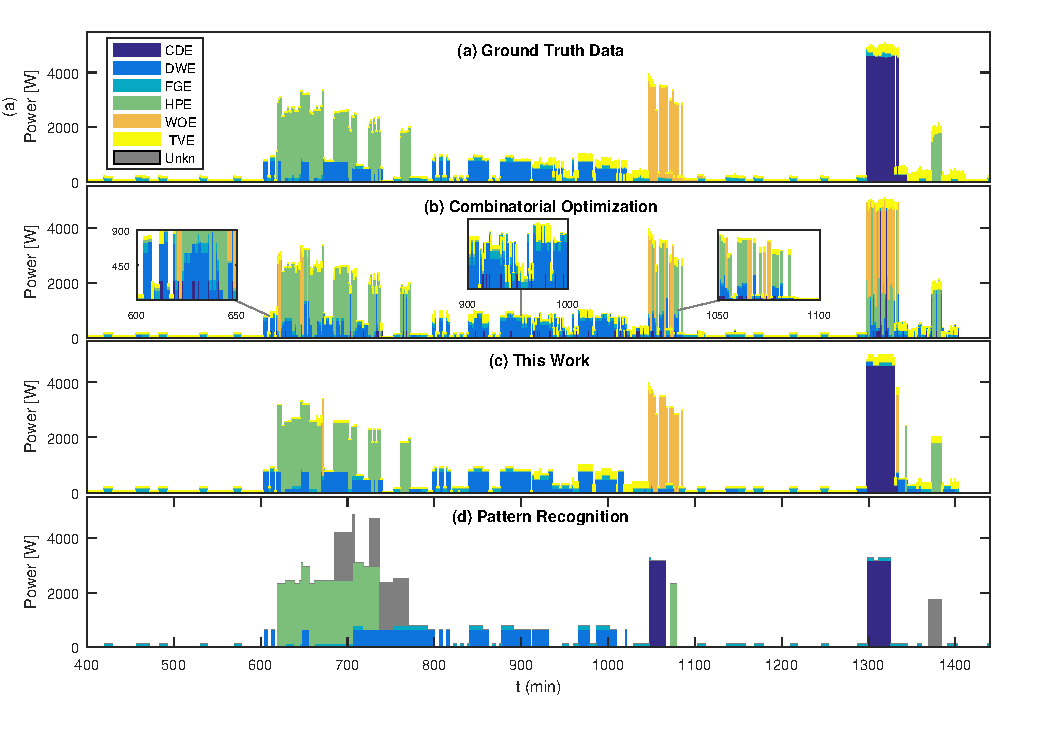
\includegraphics[width=\textwidth ]{img_test_P_2.eps}%system2.eps}
    \caption{Comparison of the real measurements (ground truth) with the proposed model and two other methods}
    \label{system2}
\end{figure*}

\subsection{Metrics}
Two metrics adapted from \cite{batra2014} are used to evaluate the accuracy of the proposed methodology. The first one will be referred as Error in Total Energy (ETE) shown in equation \eqref{metrica1}. ETE measures how well the energy consumed by each appliance was predicted. The second metric is known as Error in Assigned Power (EAP), shown in the equation \eqref{metrica2}. EAP measures how well each appliance was correctly assigned at each time slice $t$. Both metrics are normalized by the appliance's total energy consumption $y_j(t)$. The second metric provides more insight since it evaluates the correctness of the identification for each time. In other words, unlike the first metric, it does not counterbalance appliances identified at different time periods. 

\begin{equation}\label{metrica1}
   ETE_j = \dfrac{|\sum_{t}{y_j(t)} - \sum_{t}{\hat{y}_j(t)}|}{\sum_{t} { y_j(t)}}
\end{equation}

\begin{equation}\label{metrica2}
   EAP_j = \dfrac{\sum_{t} { |y_j(t) - \hat{y}_j(t)|}}{\sum_{t} { y_j(t)}}
\end{equation}


For a given appliance $j$, $y_j(t)$ is its true power measurement and $\hat{y}_j(t)$ is the predicted power at each time instant $t$. Ideally, both errors should be zero. However, it is worth mentioning that a value of zero is never achieved due to the approximation of the load signature. Hence, even in cases where the NILM algorithm detects the correct load, an error would exist. It is also worth mentioning that both metrics can achieve error rates higher than 100\%. For example, a predicted power $\hat{y}_j(t)$ higher than twice the ground truth power $y_j(t)$ can lead to such behaviour.  

\section{Tests and Results}

This section shows the results from the test cases introduced in the previous section. The MS problem is verified in CO. Also, the test case is going to be compared with Hart's pattern recognition method \cite{hart}.

\subsection{Test Case A (Active Power only)}

Results considering only the active power described in the Test Case A are discussed here. Fig.~\ref{system2} shows graphical results and compares with the two other algorithms. Table~\ref{results} shows the numerical results. The next three subtopics will discuss the behavior of each algorithm in more detail.

\subsubsection{CO Method and Verification of the MS Problem}

Fig.~\ref{system2}.b shows the disaggregation results applying only the classic CO from Algorithm \ref{algorithm1}. The highlighted zooms show a series of unrealistic activations of different loads, which is an example of the MS problem discussed in the introduction section. The first column in Table~\ref{results} shows the numerical results using the proposed metrics.  The average EAP error of the CO method is about $90\%$. 


\subsubsection{Proposed Model}
Fig.~\ref{system2}.c shows the disaggregation results using the full proposed model in the Algorithm~\ref{algorithm2}. 


%As shown in Fig. \ref{system2}.c, the multiple switching problem has been avoided by the proposed NILM method. 
The minimum time constraints \eqref{md1}-\eqref{md3} help the model to avoid multiple load switching. The second column of Table~\ref{results} shows the disaggregation results. In comparison with CO, the proposed model has a lower EAP for all loads.
%This is one of the limitations of the proposed work, since it approximates a load that is continuously switching to a continuous load.
Regarding the computational time, the usage of windows reduced the simulation time from several hours (more than 10 hours) to only a few minutes (about 3 minutes in average). FGE was the most problematic load.

\begin{table}[tb]
\centering
\caption{Error for the Case A with the Active Power Only}
\label{results}
\begin{tabular}{lcccccc}
\hline
    & \multicolumn{2}{c}{CO (\%)}                            & \multicolumn{2}{c}{This Work (\%)}                    & \multicolumn{2}{c}{Patt. Rec. (\%)}                     \\
    & \multicolumn{1}{l}{ETE} & \multicolumn{1}{l}{EAP} & \multicolumn{1}{l}{ETE} & \multicolumn{1}{l}{EAP} & \multicolumn{1}{l}{ETE} & \multicolumn{1}{l}{EAP} \\ \hline
CDE & 50.8                    & 98.2                   & 7                       & 7.3                     & 8.7                     & 84.1                    \\
DWE & 39.1                    & 89                    & 16.8                    & 29                    & 5.6                     & 74.1                    \\
FGE & 7.1                     & 70.7                    & 3.6                    & 43.9                    & 3.6                     & 53.3                    \\
HPE & 6.2                     & 57                    & 1.1                    & 5.2                    & 0.1                     & 65.9                    \\
WOE & 17.7                    & 160.1                   & 5.5                     & 15.4                    & -                       & -                       \\
TVE & 12.9                    & 55.5                    & 17.7                    & 20.7                    & -                       & -                       \\ \hline
\textbf{Average} & 22.3      & 88.41                    & 8.62                   & 20.25                   & 4.5                     & 69.35                   \\ \hline
\end{tabular}
\end{table}

\subsubsection{Comparison with Pattern Recognition}
Fig.~\ref{system2}.d shows the disaggregation results for this method. Four out of the six appliances were identified. One unknown load was also identified, which seems to be associated to the heat pump (HPE). As an example of edge dependency, the turn off event of the HPE was not detected at $t = 672$. Hence, when the load was turned on again at $t = 684$, the pattern recognition algorithm assigned the event to a different (unknown) load. The same problem also happens in the next few events and are assigned to the unknown load. The third column of the Table~\ref{results} shows the numerical results. All EAP values are over 50\%. The ETE error is lower than the other two methods; however, the ETE metric considers the energy consumption of the overall time period.

%\begin{figure}[tb]
%    \vspace{-5pt}
%    \centering
%    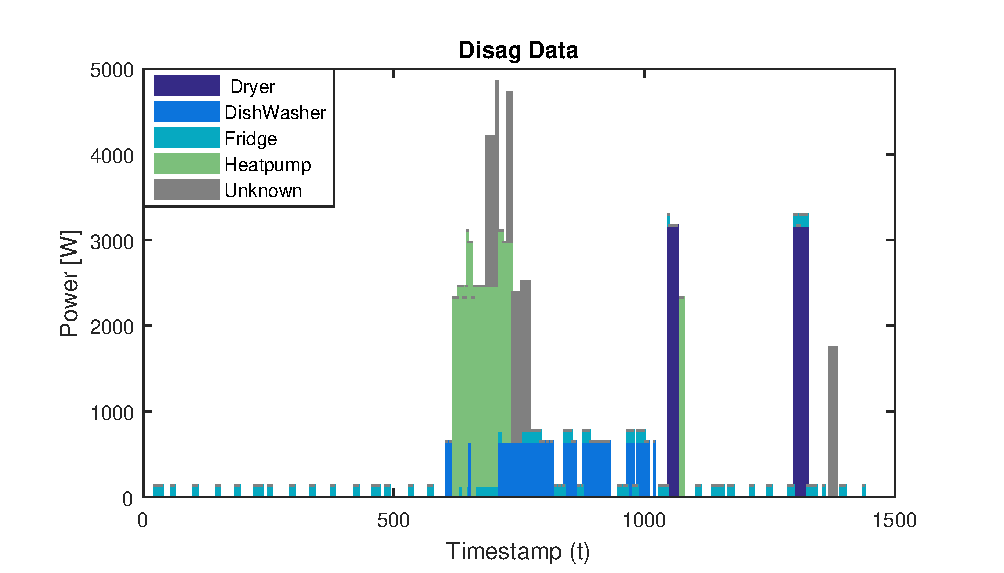
\includegraphics[width=1\columnwidth ]{results_pattern_with_unk_solo.eps}
%    \vspace{-5pt}
%    \caption{Disaggregation results applying Hart's pattern recognition algorithm.}
%    \label{hartmethod}
%\end{figure}

\subsection{Test Case B (with Reactive Power)}
The Table~\ref{results_Q} shows the numerical results when including the reactive power measurements. All the values in EAP were improved in the proposed model when comparing with the previous test case in Table~\ref{results}. Thus, the addition of new features, when available, helps on improving the method's accuracy. The average of ETE for the proposed model decreased from 8.62\% to 7\%. In addition, the average of EAP for the proposed model decreased from 20.25\% to 15.5\%. The results for CO have also highly improved from 26.65\% to 6.05\% (ETE), and from 89.7\% to 21.05\% (EAP), respectively. For pattern recognition, the same results are presented since the original method requires only reactive power.

\begin{table}[tb]
\centering
\caption{Error for the Case B Including the Reactive Power}
\label{results_Q}
\begin{tabular}{lcccccc}
\hline
    & \multicolumn{2}{c}{CO (\%)}                            & \multicolumn{2}{c}{This Work (\%)}                    & \multicolumn{2}{c}{Patt. Rec. (\%)}                     \\
    & \multicolumn{1}{l}{ETE} & \multicolumn{1}{l}{EAP} & \multicolumn{1}{l}{ETE} & \multicolumn{1}{l}{EAP} & \multicolumn{1}{l}{ETE} & \multicolumn{1}{l}{EAP} \\ \hline
CDE & 0.2                     & 0.5                     & 5.7                     & 6.1                     & 8.7                     & 84.1                    \\
DWE & 11.5                     & 28.1                    & 14                    & 23.2                    & 5.6                     & 74.1                    \\
FGE & 3.9                     & 43.5                    & 0.3                    & 28                    & 3.6                     & 53.3                    \\
HPE & 1.3                    & 5.6                    & 0.7                     & 4                     & 0.1                     & 65.9                    \\
WOE & 6.7                     & 9.5                     & 2.2                     & 12.2                    & -                       & -                       \\
TVE  & 16.1                   & 34.5                      & 19.3                    & 19.7                    & -                       & -                       \\ \hline
\textbf{Average} & 6.61       & 20.28                   & 7                     & 15.5                      & 4.5                     & 69.35                   \\ \hline
\end{tabular}
\end{table}

\subsection{Test Case C}
Table~\ref{results2} shows the numerical results for the test case C. The dataset in this case considers one more appliance than the former and a longer period of measurements. Results in Table~\ref{results2} show an EAP of 24.97\% which is almost half of the error from the other compared methods. The pattern recognition strategy identified three of the seven appliances. The most problematic appliances were DWE and FGE, with EAP of 54.7\% and 39.9\% respectively. However, error is still lower than for the other two compared methods. 

\begin{table}[tb]
\centering
\caption{Error for the Case C for a Longer Period}
\label{results2}
\begin{tabular}{lcccccc}
\hline
    & \multicolumn{2}{c}{CO (\%)}                            & \multicolumn{2}{c}{This Work (\%)}                    & \multicolumn{2}{c}{Patt. Rec. (\%)}                     \\
    & \multicolumn{1}{l}{ETE} & \multicolumn{1}{l}{EAP} & \multicolumn{1}{l}{ETE} & \multicolumn{1}{l}{EAP} & \multicolumn{1}{l}{ETE} & \multicolumn{1}{l}{EAP} \\ \hline
BME & 0.4                   & 36.8                  & 5.9                   & 22.2                  & -                    & -                    \\
CDE & 0.2                   & 2.8                   & 4.7                   & 12.2                  & 42.8                 & 52.2                   \\
DWE & 32.2                  & 109.3                   & 14.8                  & 54.7                  & -                    & -                    \\
FGE & 43.6                  & 83.2                  & 9.4                   & 39.9                  & 15.4                 & 64.1                   \\
FRE & 27                    & 27.3                  & 11.8                  & 12.2                  & -                    & -                       \\
HPE & 2.8                   & 6                   & 2.7                   & 4                   & 3.6                  & 16.1                   \\ 
TVE & 51.2                  & 94.2                  & 10                    & 29.6                  & -                    & -                    \\ \hline
\textbf{Average} & 22.48     & 51.37                  & 8.47                   & 24.97                  & 20.6                 & 44.1                 \\ \hline
\end{tabular}
\end{table}

%\section{Unsupervised Tests}

\section{Summary and Analysis of Results}
This chapter presented the experiments for both the supervised and unsupervised setting. A public dataset was considered for the supervised setting while a local private dataset for the unsupervised one. As discussed in \cite{zeifman_analysis}, a good NILM algorithm should address the following six requirements: use typical meter features, minimal accuracy, no training, real-time capability, scalability, and flexibility.

The presented NILM algorithm accomplishes with most of the former requirements, since: uses only low frequency features; accomplishes the minimum 80\% requirement (considering the complement of ETE's average); the parameters in the input table make it suitable for a no training (unsupervised) setting; the results could be shown in real-time to the user at every $m$ measurements; scalability will depend on the way in which the input table is constructed and how it is updated; finally multiple appliances types are handled (multi-state, ON/OFF, constant) thanks to the parameters $MD_i$ and $prev_i$. 

    
    
\chapter{Conclusion}
In this dissertation, a NILM method based on MILP optimization was proposed. The classic CO model was expanded for increasing the accuracy and performance. As main contribution, a new set of integer linear constraints to efficiently model the behaviour of appliances' load signature was presented. Also, a window-based algorithm is proposed in order to enhance the computational complexity. The proposed algorithm surpassing the test cases for the identification of appliances. As main advantage, the algorithm does not require data in high resolution, hence low-cost smart meters are sufficient to deploy it. Results were accomplished with a one-minute reading resolution. The usage of windows proved to be effective in limiting the complexity growth. In addition, the inclusion of other features besides the active power is optional and help to improve the accuracy. Finally, the table of parameters is suitable to an unsupervised approach. 

\iffalse

\section{Future directions}
The following list shows points that might be considered for future work in this area

\begin{itemize}
\item Communication of time between windows: What could help is to implement an intermediary window. For example, if the window size is 10, we could make the solver run every 5 measurements ahead. 
\item Implement probabilistic functions: for example, penalization for turning on on unlikely times (like a washing machine at 3 AM). 
\item Implement the concept of occupied and non-occupied type of loads: Associate a low probability of human operated appliances during the dawn. 
\end{itemize}
\fi
    
    % Ordem final: Referencias, apendices e anexos
    \printbibliography
    
    % – Implementação, Resultados, Arquivos diversos, etc


\appendix
\chapter{Full Proposed Mathematical Model}

The full proposed model in details for a window based case is presented in the next page of this Appendix. The algorithm was implemented using the mathematical programming language AMPL with the very same equations.

\begin{algorithm}[htb]\label{full_model}
\SetAlgoLined
 \Repeat{$T_0$ > $T_f$}{

let  $\tilde{T} = \left\{T_{0}, \cdots, T_{0}+m \right\}$

solve
$$\min_{x_i(t)} \quad \sum_{t\ \in\ \tilde{T}} \delta_P(t) + \delta_Q(t)$$

s. t. 
%\begin{center}

\begin{equation}
P(t) - \sum_{i\ = 1}^{n} x_i(t)\ P_i \ \leq \ \delta_P(t)
\end{equation}

\begin{equation}
P(t) - \sum_{i = 1}^{n} x_i(t)\ P_i \ \geq \ -\delta_P(t)
\end{equation}

\begin{equation}
Q(t) - \sum_{i\ = 1}^{n} x_i(t)\ Q_i \ \leq \ \delta_Q(t)
\end{equation}

\begin{equation}
Q(t) - \sum_{i = 1}^{n} x_i(t)\ Q_i \ \geq \ -\delta_Q(t)
\end{equation}

\begin{equation}
x_i(t) = 0 \quad \forall t \in \tilde{T}, i \in S \ | \ P(t) \leq TH
\end{equation}

\begin{equation}
 x_i(t) - x_i(t-1) = up_i(t) - dw_i(t) \quad \forall i \in S, t > T_0
\end{equation}

\begin{equation}
 x_i(T_0) - X_i = up_i(t) - dw_i(t) \quad \forall i \in S, t = T_0
\end{equation}

\begin{equation}
up_i(t) + dw_i(t) \leq 1 \quad \forall i \in S, t \in \tilde{T}
\end{equation}

\begin{equation}
    up_i(t) = dw_{\text{prev}_i}(t) \quad \forall i \in S, t \in \tilde{T} \ | \ \text{prev}_i>0
\end{equation}

\begin{equation}
    \sum_{k\ =\ T_0}^{G_i} \left[ 1 - x_i(k) \right] = 0 \quad \forall i \in S
\end{equation}

\begin{multline}
 \qquad \qquad \qquad \qquad    \sum_{k\ =\ t}^{t+MD_i-1} x_i(k) \geq MD_i \left[ x_i(t) - x_i(t-1) \right] \\
    \forall i \in S, t \in G_i + T_0 \hdots T_f - {MD}_i + 1
\end{multline}

\begin{multline}
 \qquad \qquad \qquad \qquad \sum_{k\ =\ t}^{T_f} \left\{ x_i(k) - \left[ x_i(t) - x_i(t-1) \right] \right\} \geq 0 \\
    \forall i \in S, t \in T_f - MD_i + 2 \hdots T_f
\end{multline}
 
%\end{center}

let $T_0 = T_0 +m$ + 1
 }
\caption{Full proposed model in details.}
\end{algorithm}


\end{document}
